\documentclass[10pt,a4paper]{article}
\usepackage{amsmath}
\usepackage{amsfonts}
\usepackage{amssymb}
\usepackage[english]{babel}
\usepackage{float}
\usepackage[left=2cm,right=2cm,top=2cm,bottom=2cm]{geometry}
\usepackage{graphicx}
\usepackage{hyperref} % Used for external links
\usepackage[utf8]{inputenc}
\usepackage{listings} % Used for source code listing

% Source code listing's parameters
\lstset{
  frame=single,
  keepspaces=true,
%  title=\lstname
}

\title{First SPICE Exercise\\{\small{Fundamentals Of Electronics - a.a. 2018-2019 -
University of Padua (Italy)}}}
\author{Pietro Prandini (mat. 1097752)}

\begin{document}
\maketitle

% License
\begin{center}
\tiny{This work is licensed under the Creative Commons Attribution-ShareAlike
 4.0 International License. To view a copy of this license, visit
 \href{http://creativecommons.org/licenses/by-sa/4.0/}{http://creativecommons.org/licenses/by-sa/4.0/}
or send a letter to Creative Commons, PO Box 1866, Mountain View, CA 94042,
USA.}
\end{center}

\section{Audio amplifier}
\subsection{Voltage gain and frequency domain - Ideal op. amp.}
\begin{figure}[h]
  \centering
  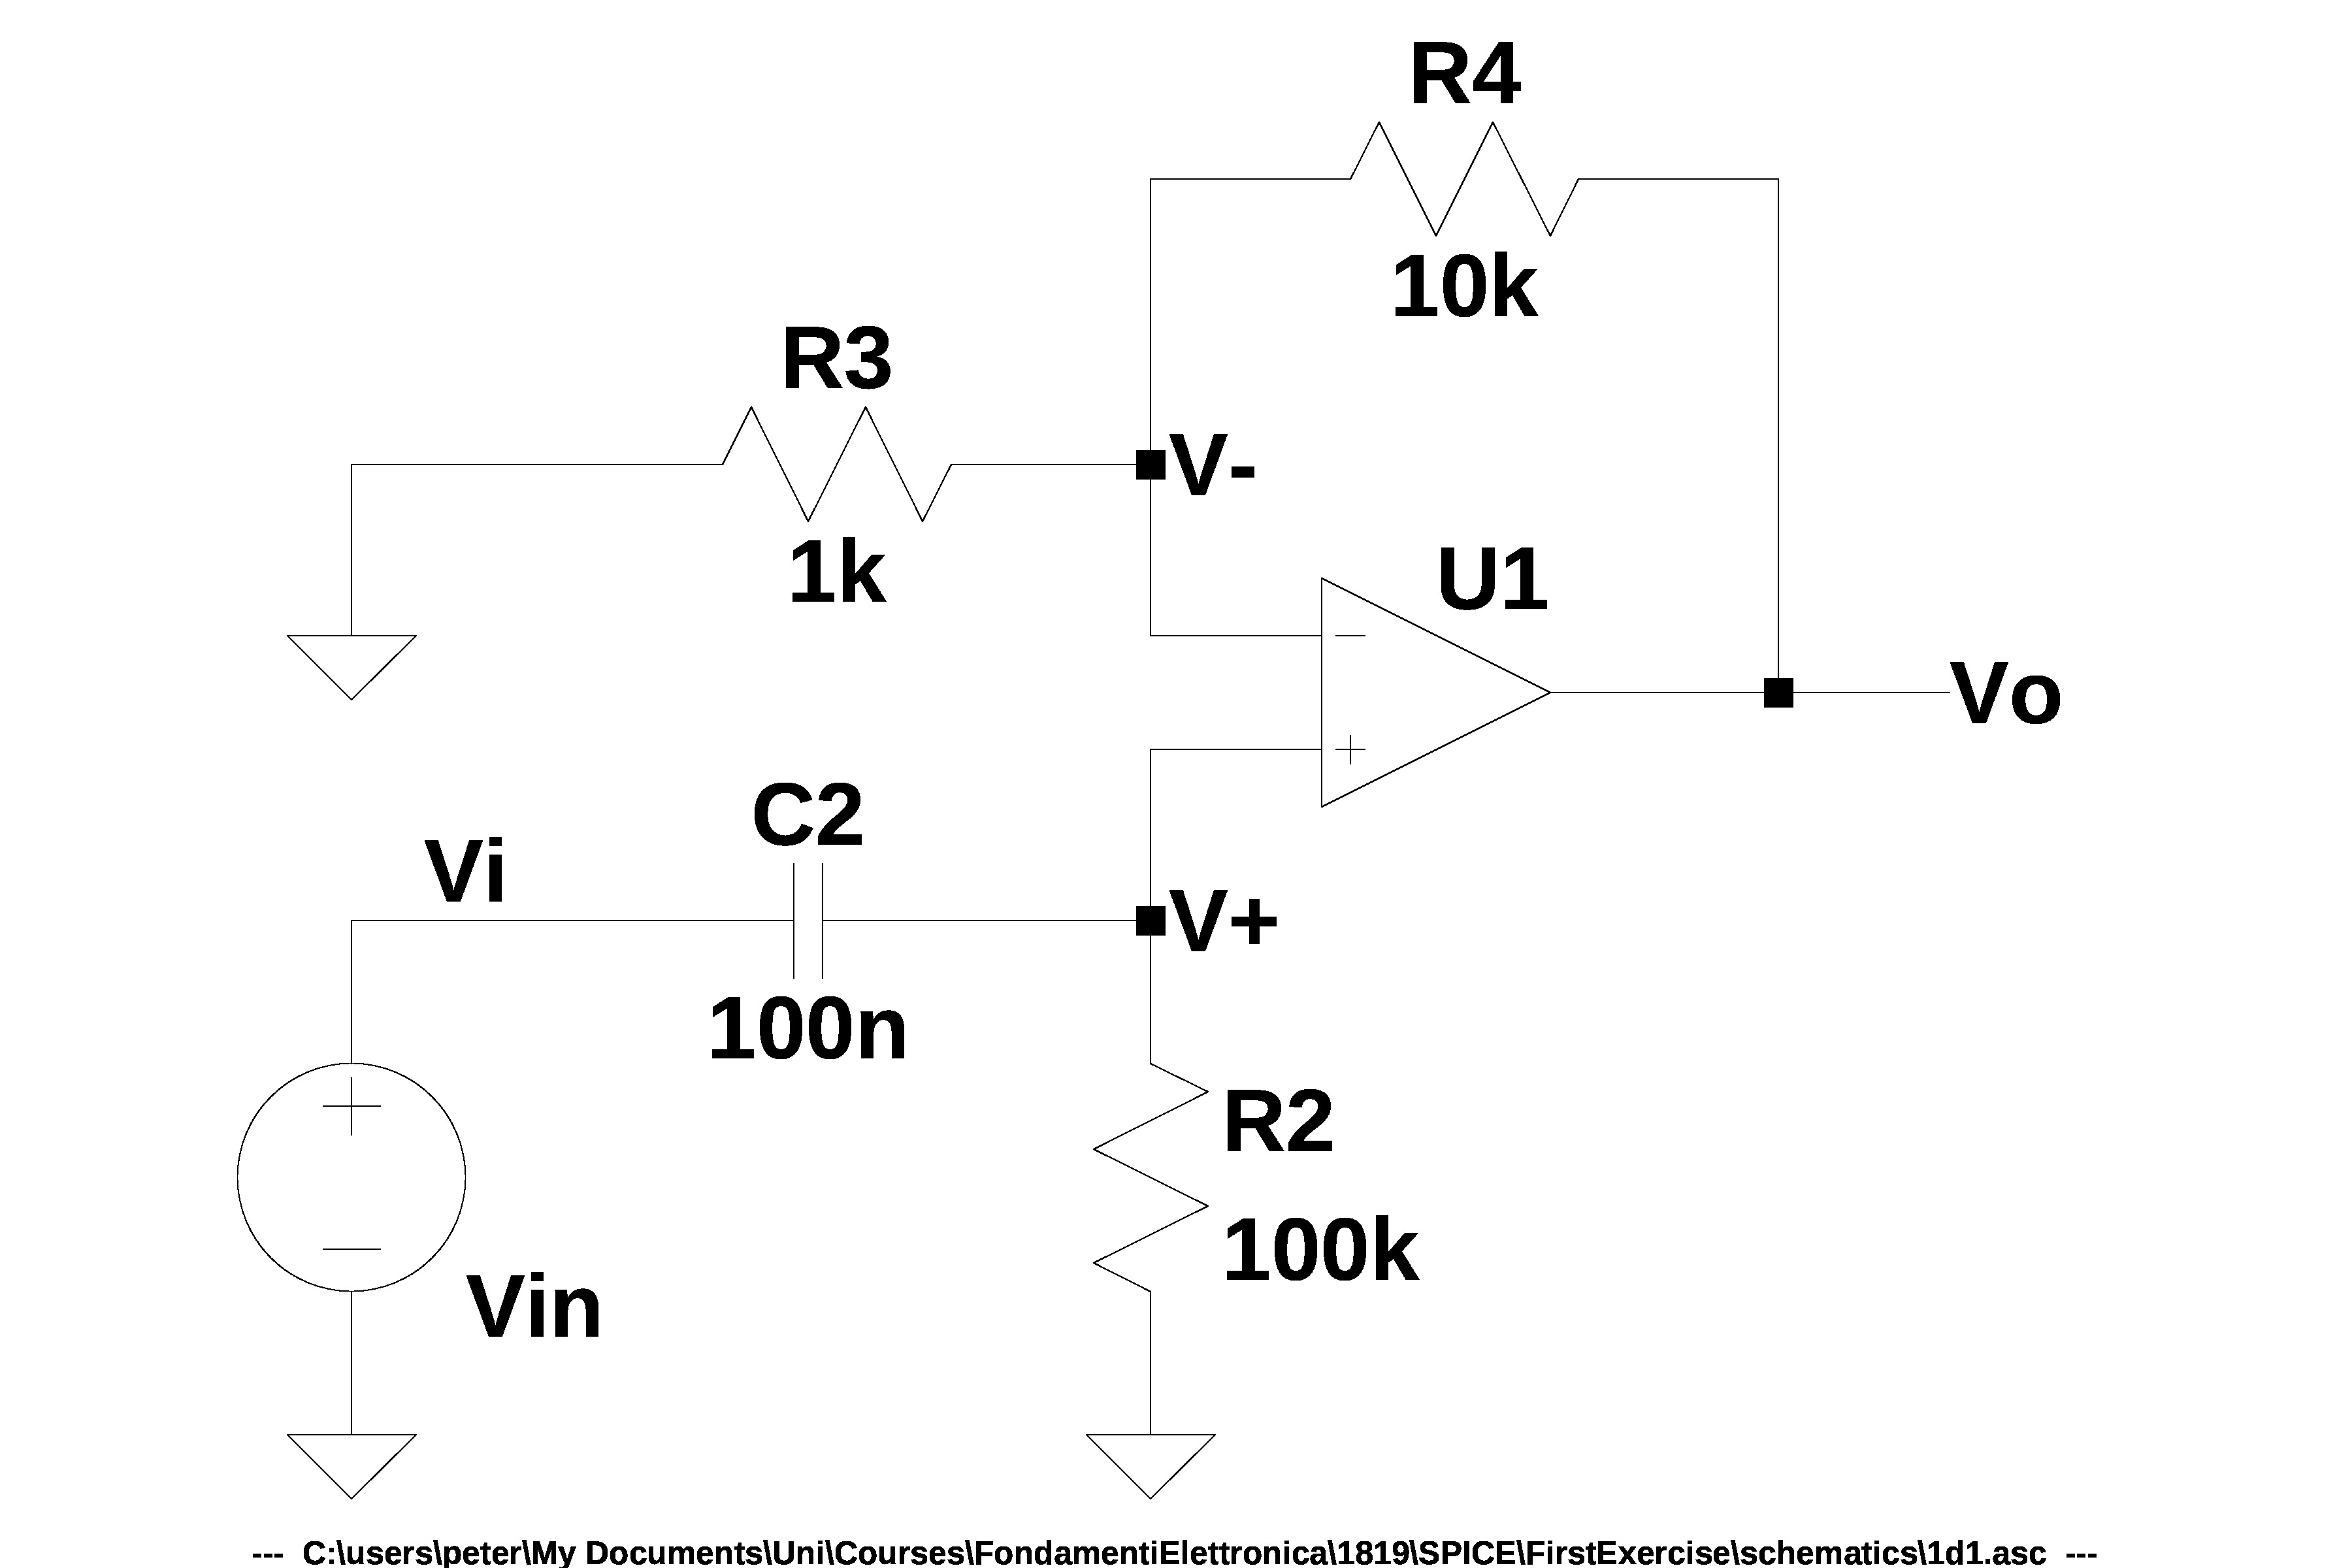
\includegraphics[width=8cm]{schematics/1d1.jpg}
  \caption{Audio amplifier - Ideal op. amp.}
  \label{1d1schematics}
\end{figure}

\begin{equation} \label{eq:V_+}
V_+ = V_{in}\frac{R_2}{R_2+\frac{1}{sC_2}} =
V_{in}\frac{R_2}{R_2+\frac{1}{sC_2}}\frac{sC_2}{sC_2} =
V_{in}\frac{sC_2R_2}{1+sC_2R_2}
\end{equation}

\begin{equation} \label{eq:V_-}
V_- = V_+
\end{equation}

\begin{equation} \label{eq:I_R3}
I_{R_3} = \frac{V_-}{R_3} = \frac{V_+}{R_3}
\end{equation}

\begin{equation} \label{eq:I_R4}
I_{R_4} = I_{R_3}
\end{equation}

\begin{equation} \label{eq:V_o}
V_o = V_+ + R_4I_{R_4} = V_+ + R_4 I_{R_3} = V_+ + R_4 \cdot \frac{V_+}{R_3} =
V_+ \cdot \left(1 + \frac{R_4}{R_3} \right) =
V_{in}\frac{sC_2R_2}{1+sC_2R_2} \cdot \left(1 + \frac{R_4}{R_3} \right)
\end{equation}

\begin{equation} \label{eq:TF}
\frac{V_o}{V_{in}} = \frac{sC_2R_2}{1+sC_2R_2}\left(1+\frac{R_4}{R_3}\right)
\end{equation}

\begin{equation} \label{eq:K}
K = C_2R_2 \cdot \left(1+\frac{R_4}{R_3}\right)
\end{equation}

\begin{equation} \label{eq:omega_1}
 \omega_1 = \frac{1}{C_2R_2}
\end{equation}

\begin{equation} \label{eq:TFBode}
\frac{V_o}{V_{in}} = K \frac{s}{1+\frac{1}{\omega_1}}
\end{equation}

\begin{equation} \label{eq:KdB}
 K|_{dB} = 20\log_{10}|K| = \log_{10}\left|C_2R_2 \cdot \left(1+\frac{R_4}{R_3}\right)\right| = -19.1722 dB
\end{equation}

\begin{equation} \label{eq:omega_1log}
\log_{10} |\omega_1| =
\log_{10} \left| \frac{1}{C_2R_2} \right|= 2.0000
\end{equation}

\subsection{Voltage output waveform - LT1028 op. amp.}
\begin{figure}[h]
  \centering
  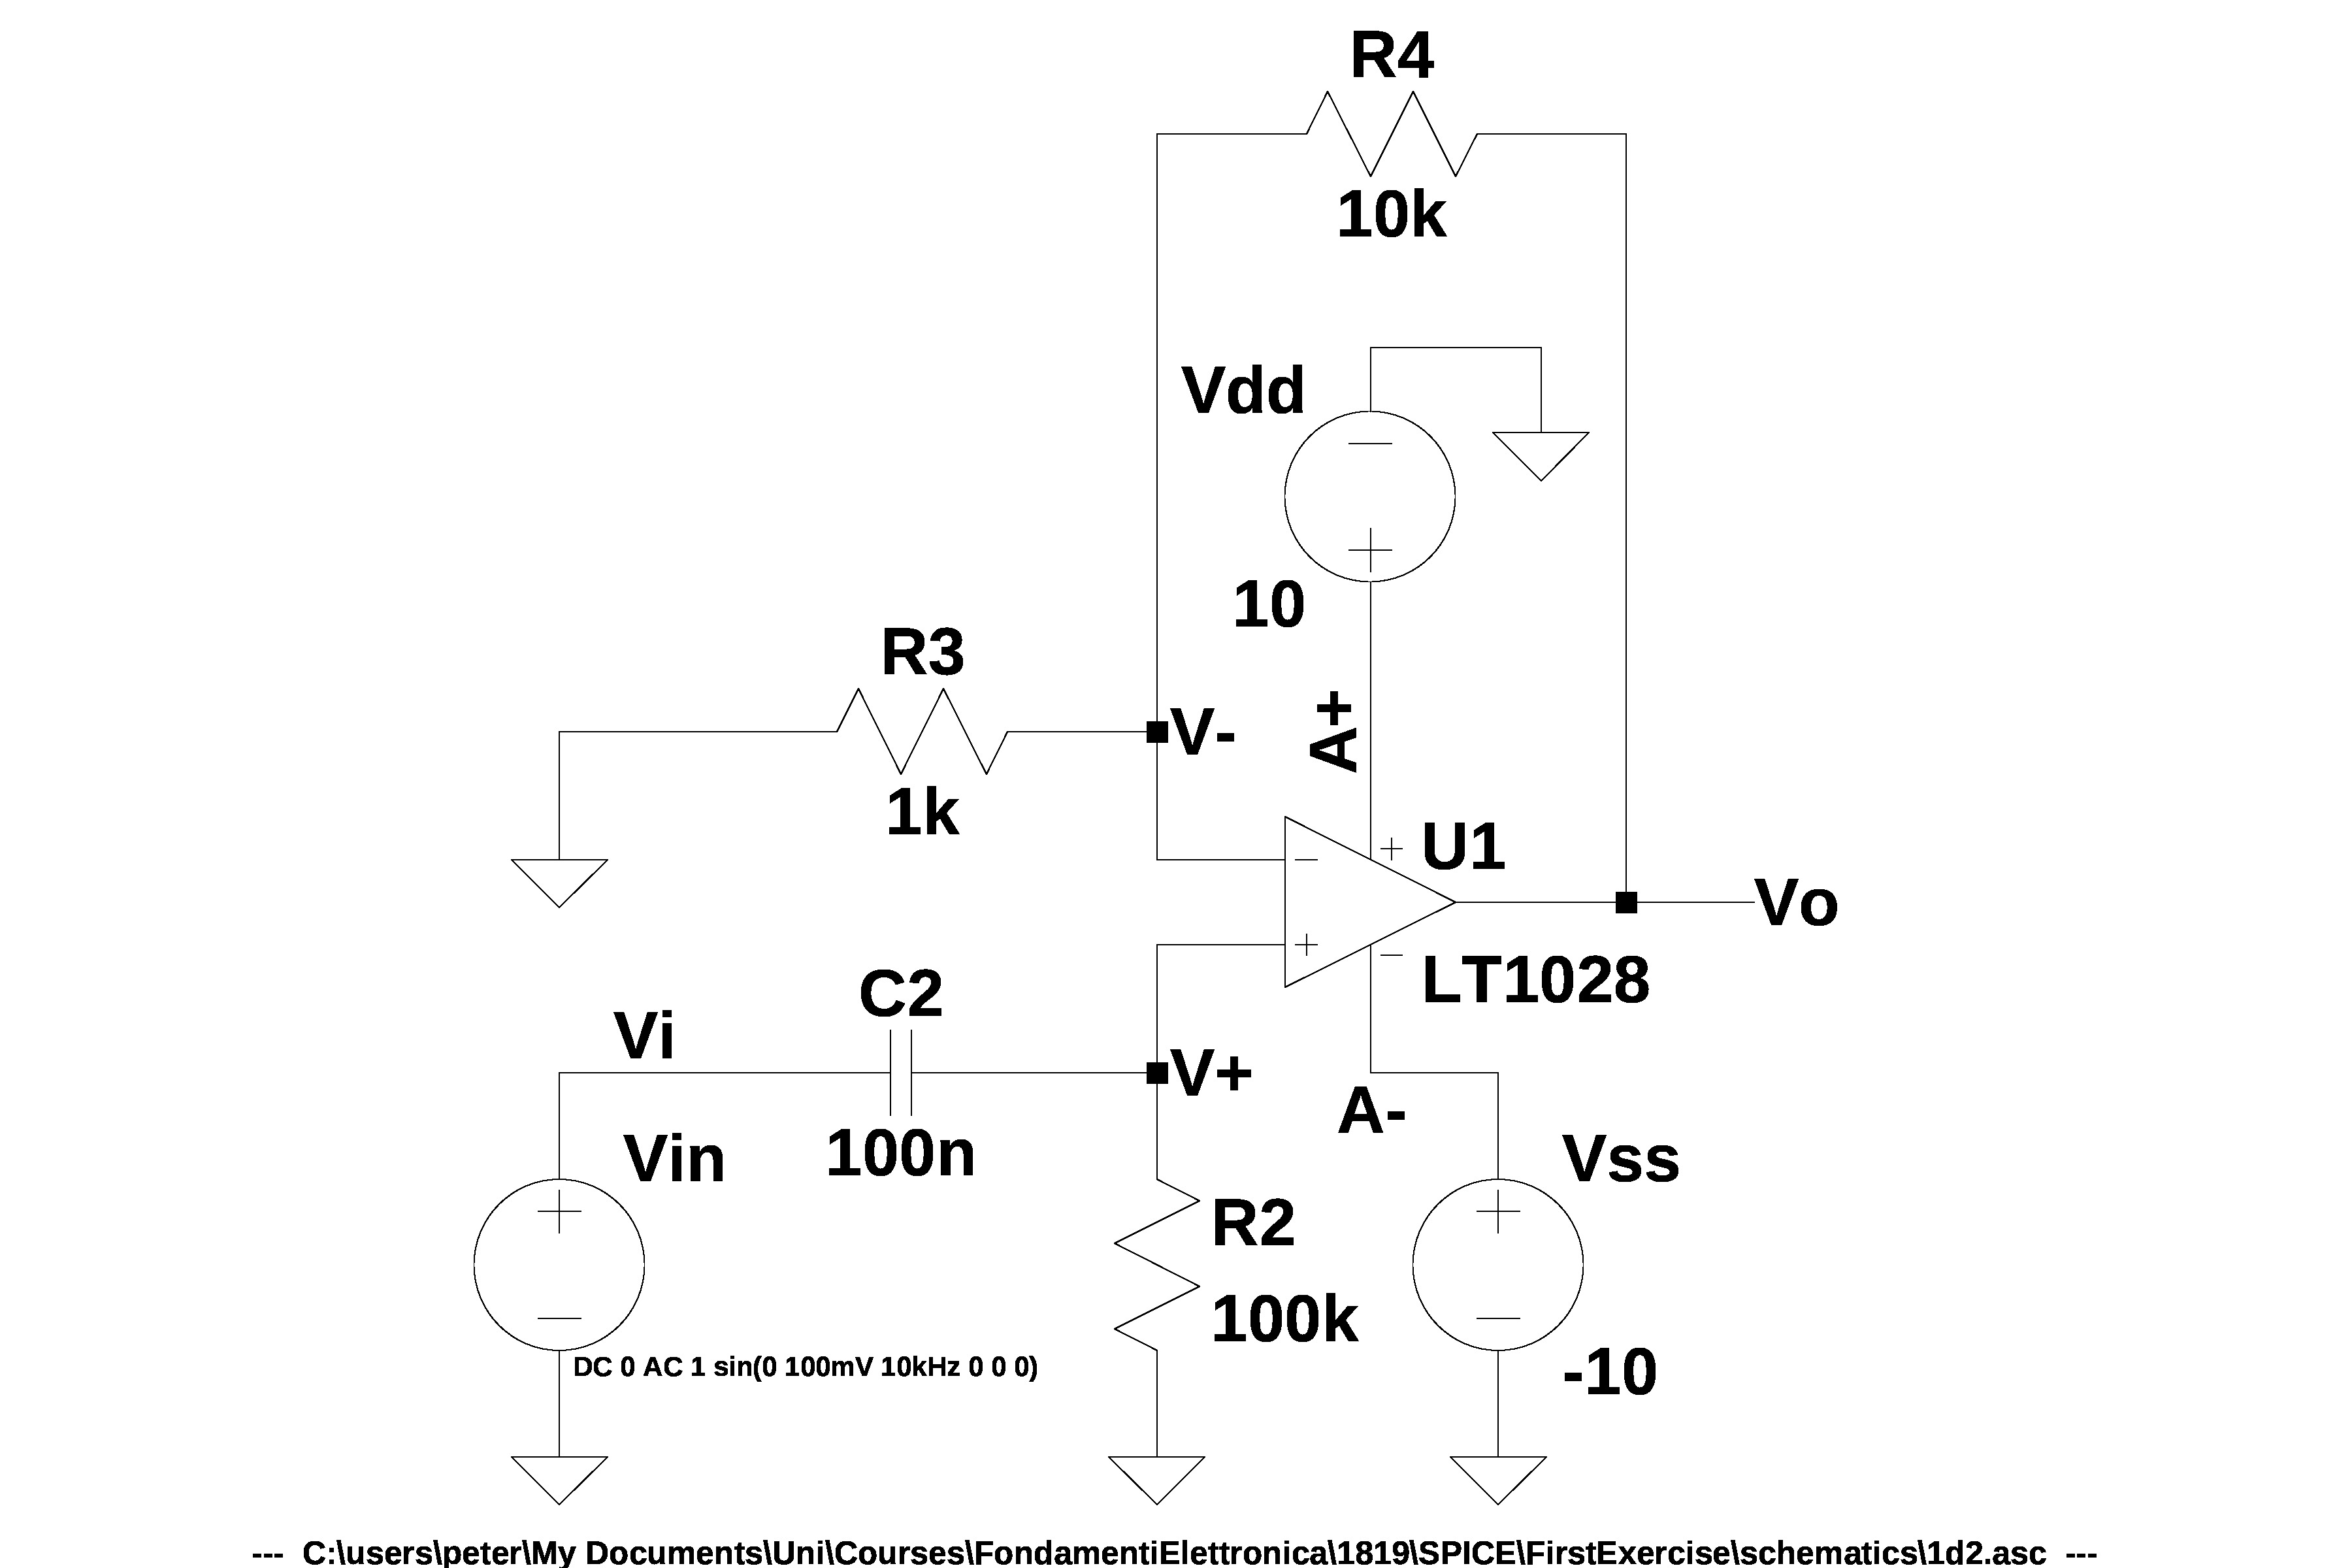
\includegraphics[width=10cm]{schematics/1d2.jpg}
  \caption{Audio amplifier - LT1028 op. amp.}
  \label{1d2schematics}
\end{figure}

\subsubsection{Netlist}
\lstinputlisting{netlist/1d2.cir}

\subsubsection{Graph}
\begin{figure}[H]
  \centering
  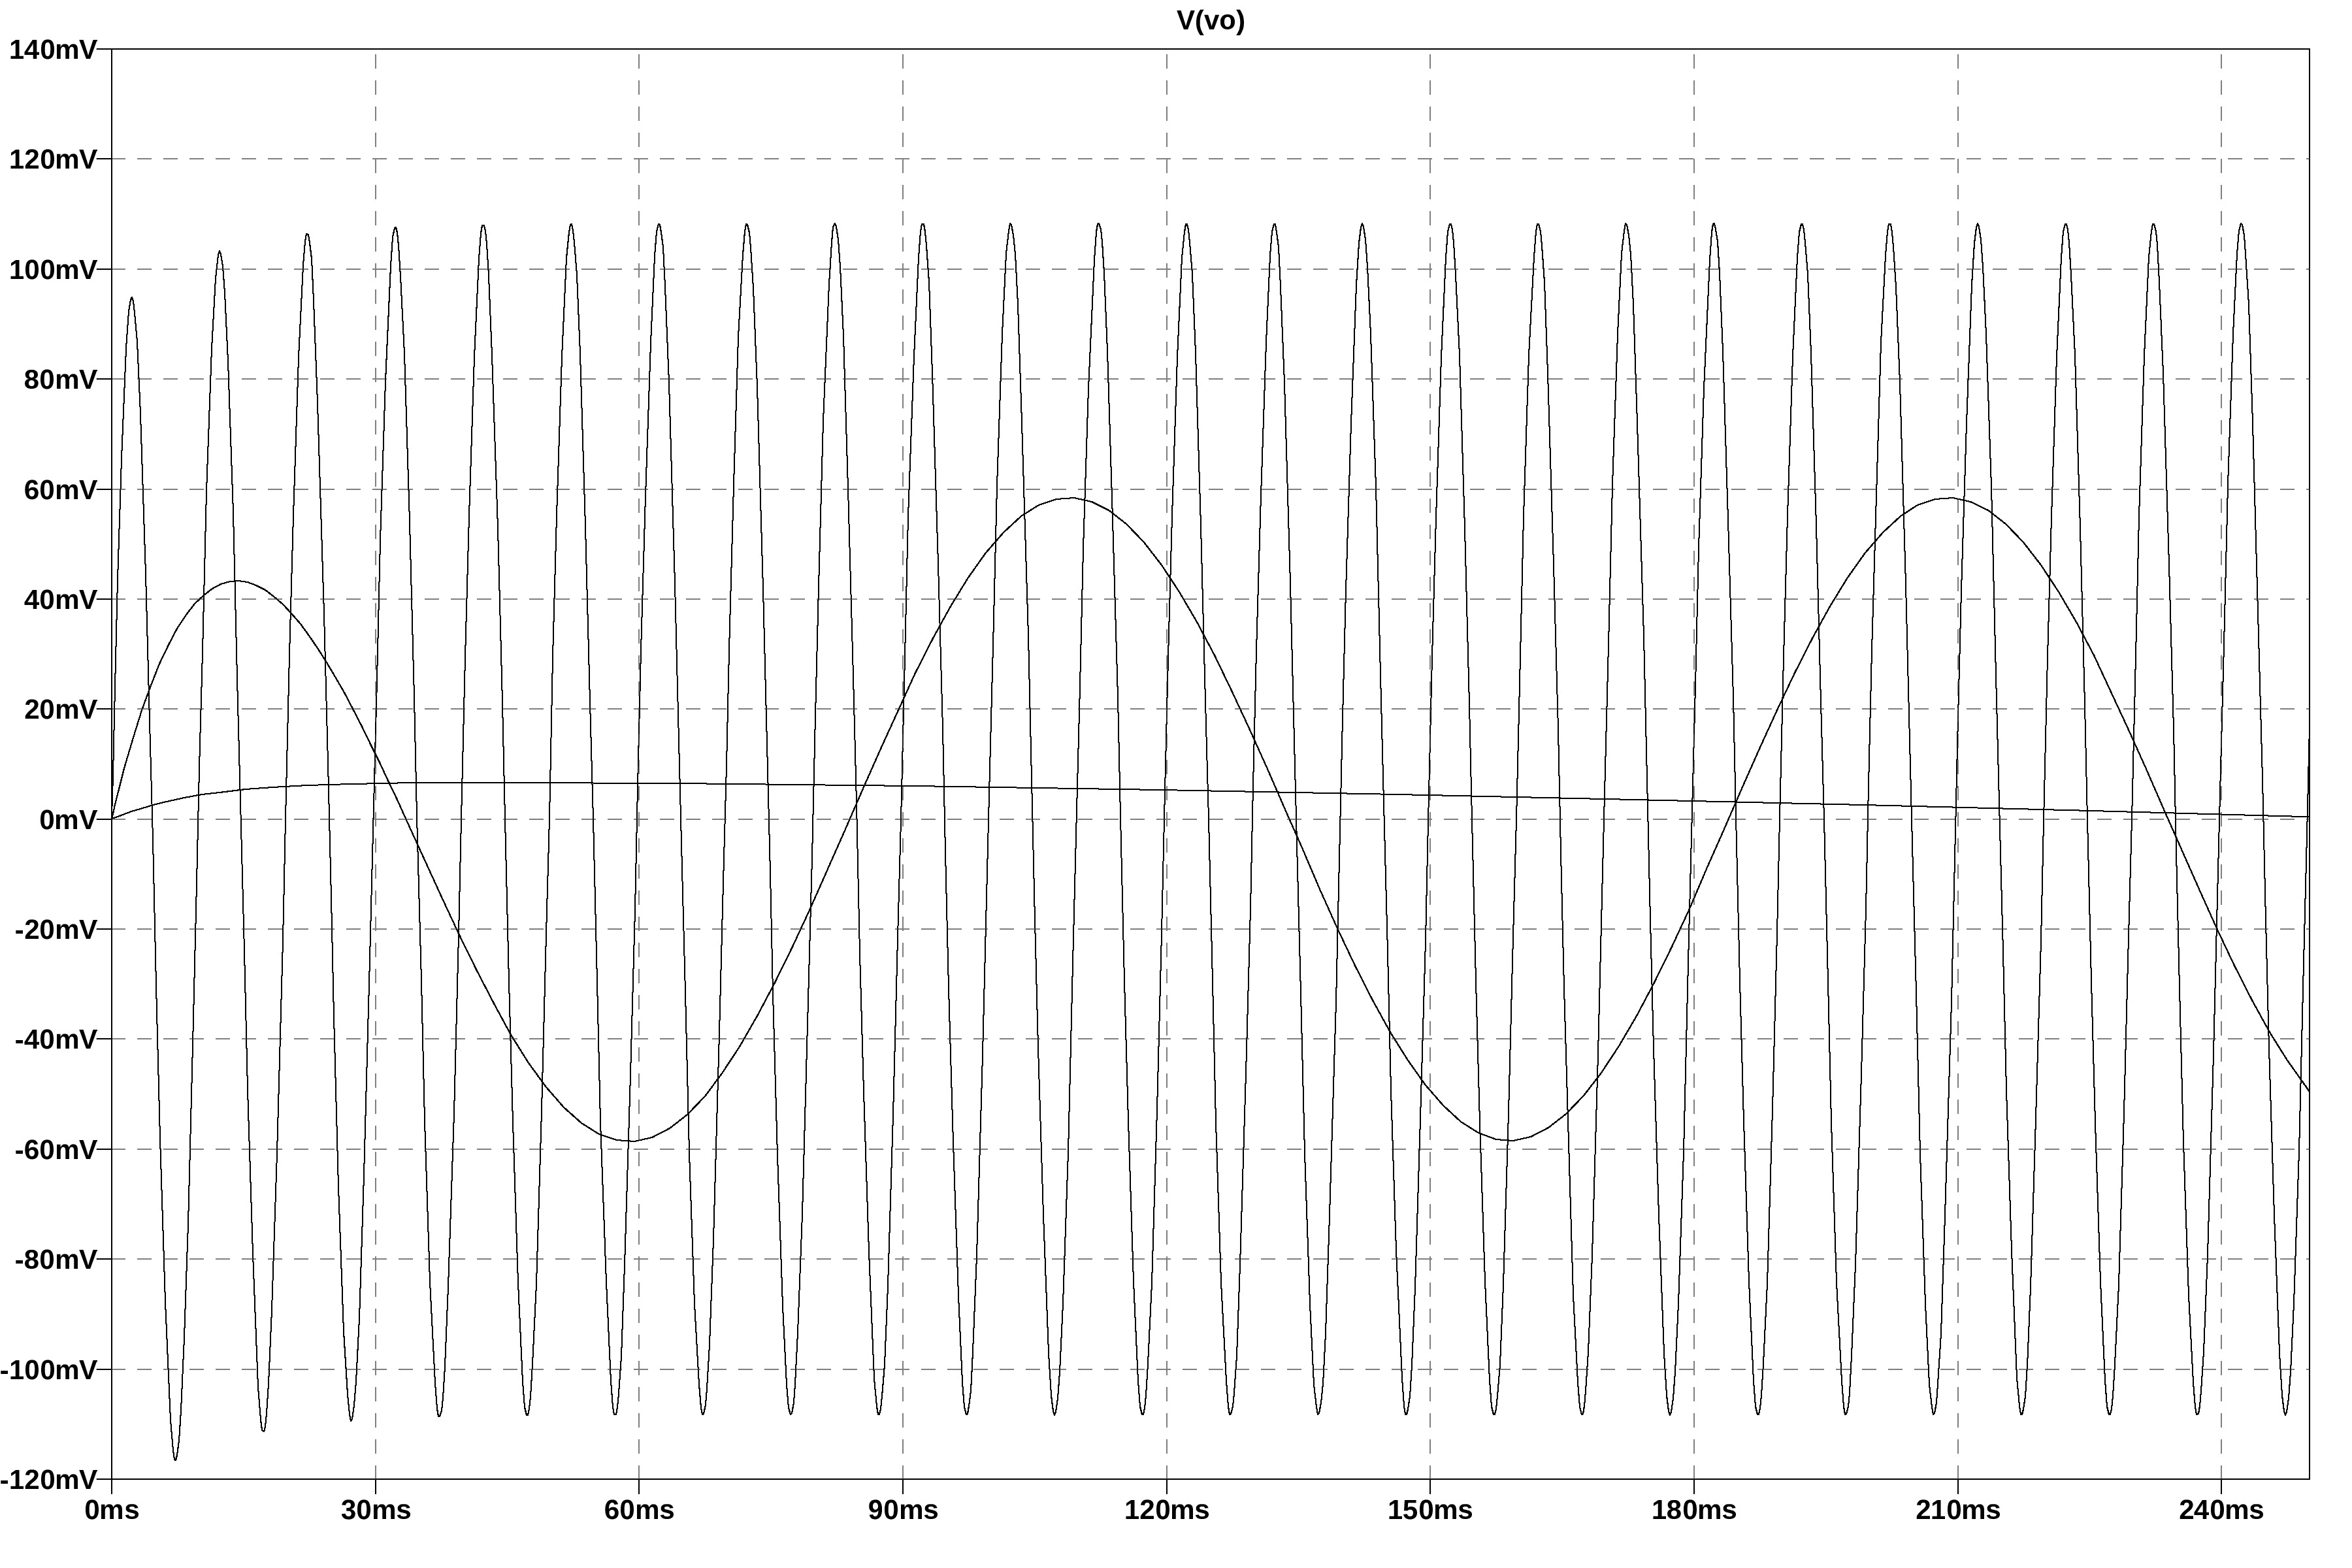
\includegraphics[width=14cm]{graph/1d2.jpg}
  \caption{Audio Amplifier - Voltage output waveform}
  \label{1d2graph}
\end{figure}

\subsection{Bode diagram - LT1028 op. amp.}
\subsubsection{Netlist}
\lstinputlisting{netlist/1d3.cir}

\subsubsection{Graph}
\begin{figure}[H]
  \centering
  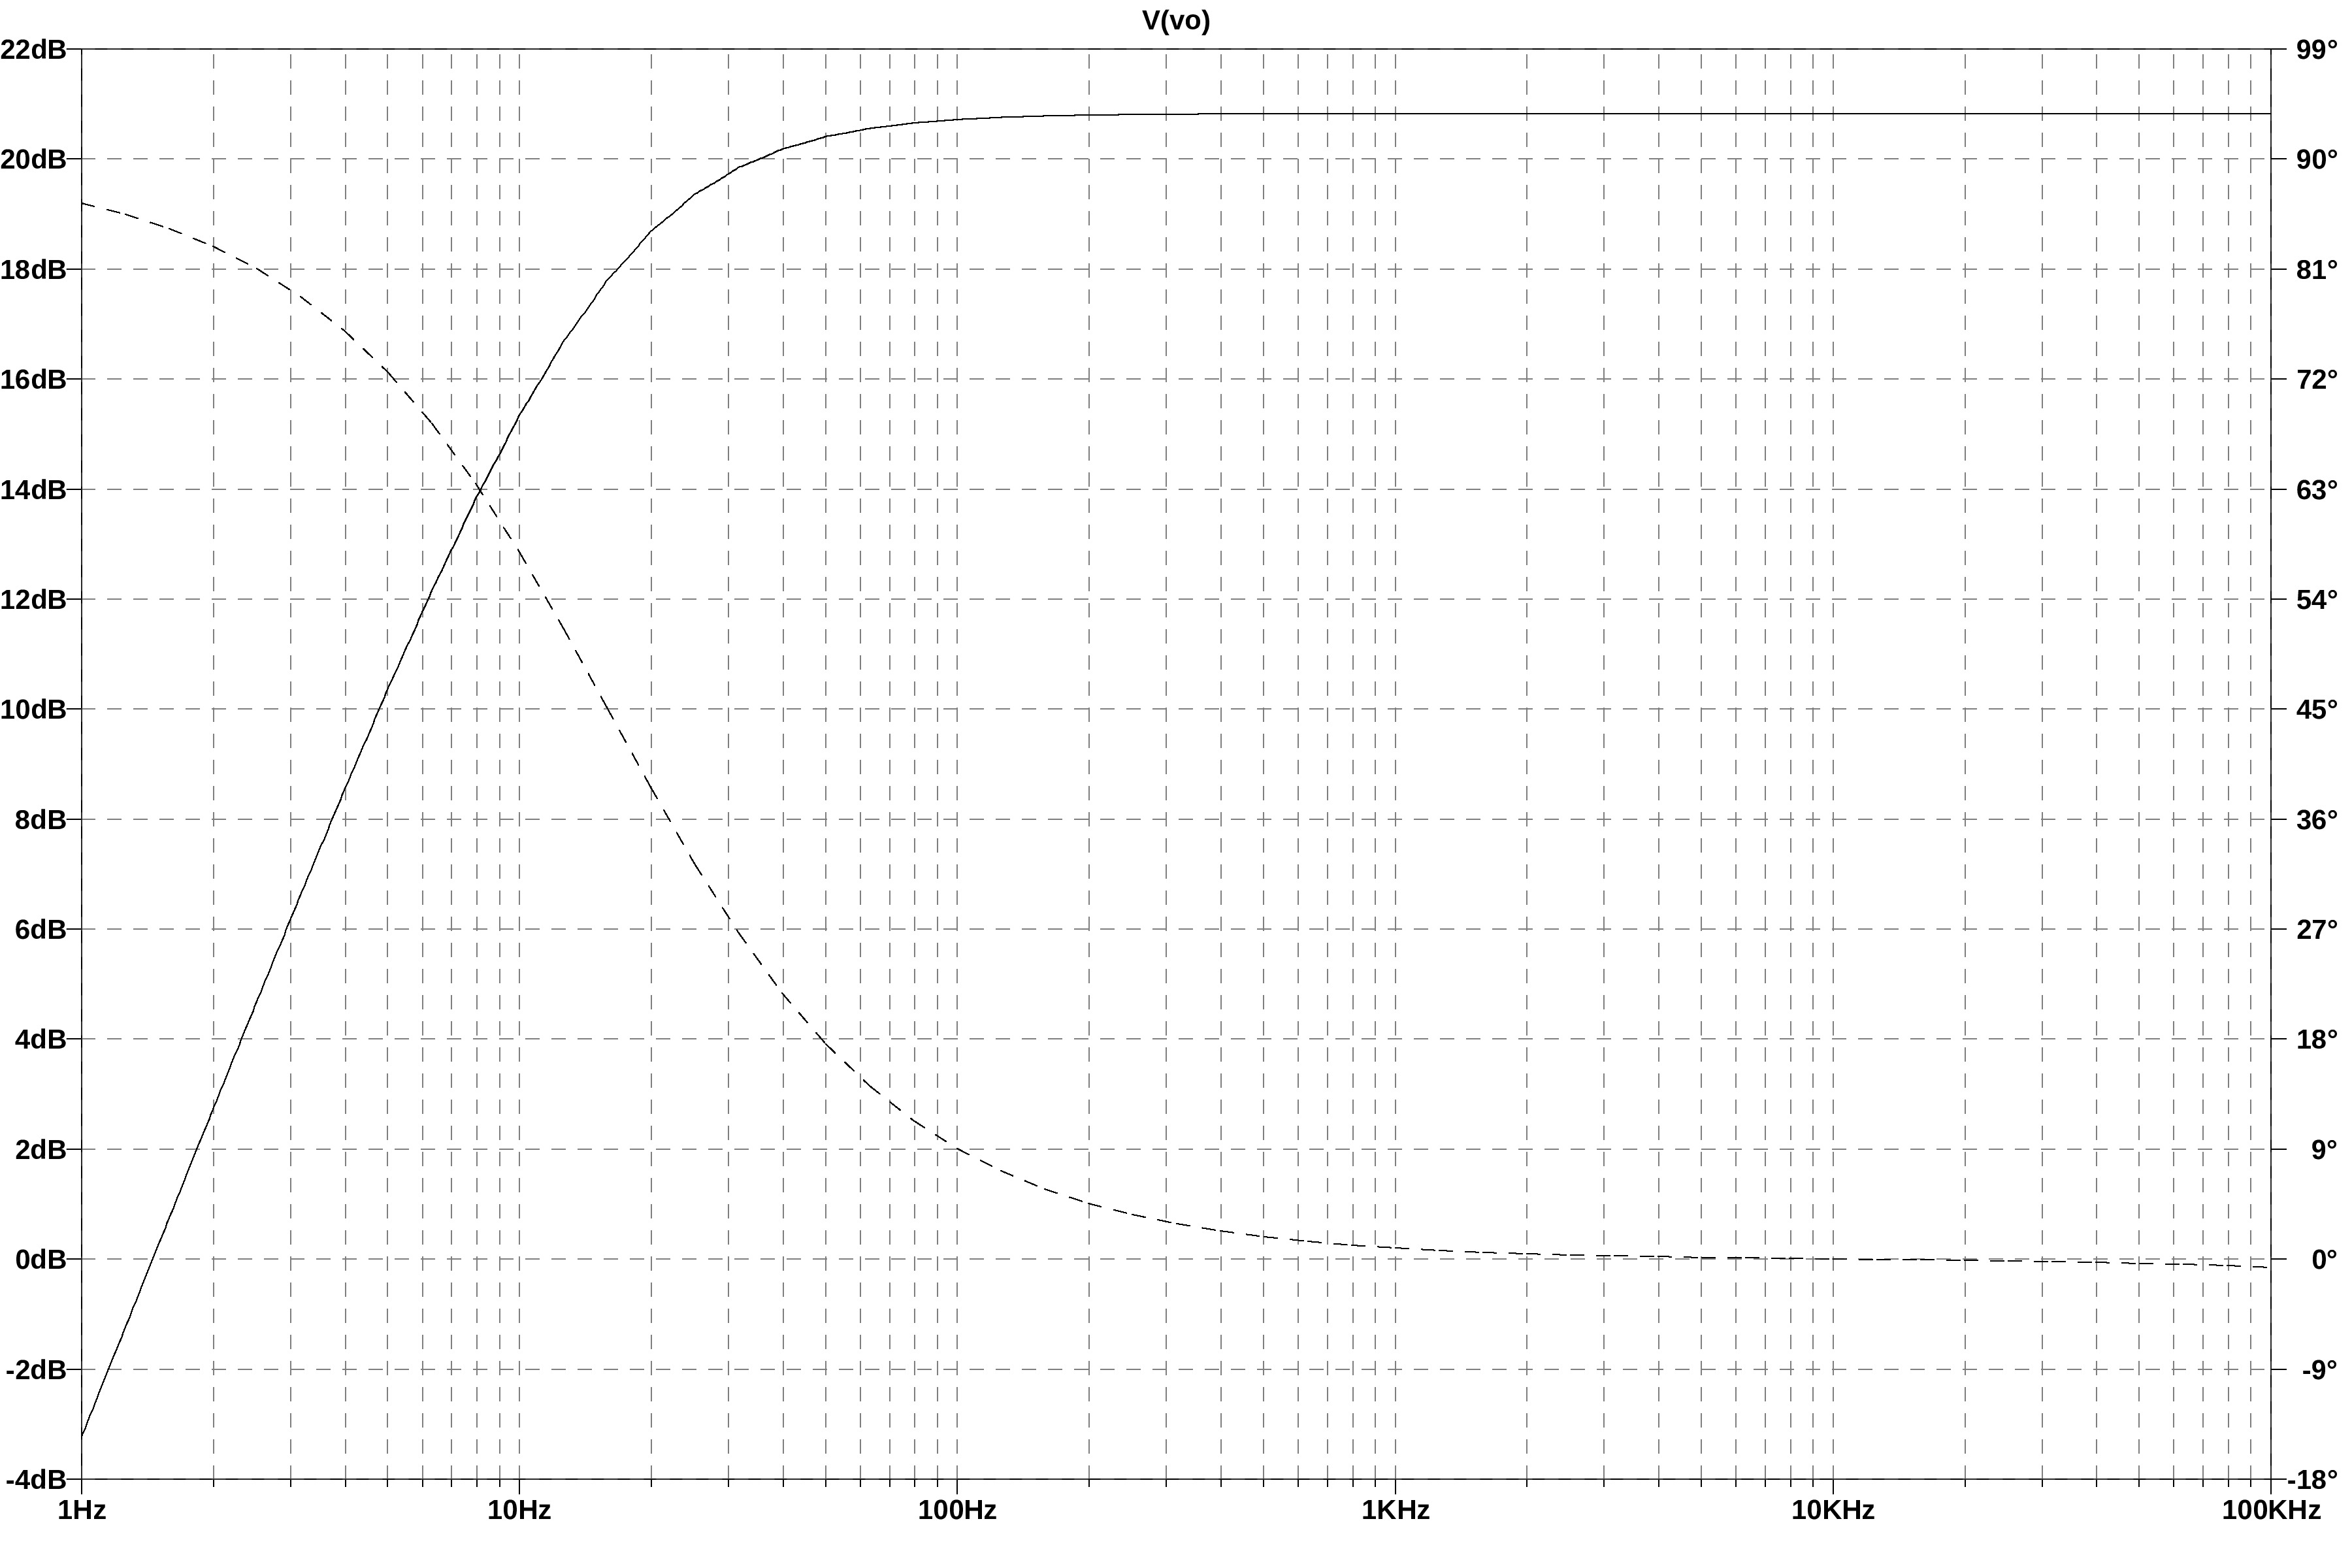
\includegraphics[width=14cm]{graph/1d3.jpg}
  \caption{Audio Amplifier - Bode diagram}
  \label{1d3graph}
\end{figure}

\end{document}
